\documentclass{report}

\usepackage{import}
\usepackage{preamble}
\usepackage{xcolor}
\usepackage{hyperref}

\title{Methods of Spectr analyses}
\author{sukhanov.mikle }
\date{September 2020}


 
 % Цвета для гиперссылок
\definecolor{linkcolor}{HTML}{799B03} % цвет ссылок
\definecolor{urlcolor}{HTML}{FF0000} % цвет гиперссылок
 
\hypersetup{pdfstartview=FitH,  linkcolor=linkcolor,urlcolor=urlcolor,  colorlinks=true} %отображение ссылок цветом а не рамкой

% \newcommand{\wcc}{WinCC OA}
% \newcommand{\jcp}{JCOP framework}
% \newcommand{\folder}[1]{\textbf{\ttfamily #1}}
\newcommand{\bi}{\begin{itemize}}
\newcommand{\ei}{\end{itemize}}
\newcommand{\be}{\begin{equation}}
\newcommand{\ee}{\end{equation}}
\newcommand{\vx}{$\vec{x}$}

\begin{document}

%\maketitle
\begin{Large}


\section*{Введение}
Одной из самых распространенных задач анализа функциональных зависимостей является необходимость нахождения максимума (минимума) или как говорят <<экстремума>> функции. Из школьного курса известно, что точка экстремума функции $f(x)$ находится из простейшего уравнения:
\be
f'(x) = 0
\label{extremum}
\ee
Однако при поиске экстремума в экспериментальных зависимостях, полученных тем или иным путем, мы можем столкнуться со следующими проблемами:
\bi
\item Уравнение (\ref{extremum}) трансцендентное, то есть не имеет аналитического решения.
\item Функция не может описываться аналитически, то есть нет математического выражения, которое могло бы описать данную зависимость.
\ei

Поскольку в реальном мире мы не можем наблюдать непрерывные функциональные зависимости, все функции считаются дискретными. Для нахождения экстремумов таких функций используются методы, основанные на численных методах, то есть которые могут быть <<загнаны>> в код программы и выполнены для обработки различных данных. 

В общем случае любые полученные данные в зависимости от какой либо переменной на этапе эксперимента напоминают черный ящик. То есть на каждый набор входных параметров $\vec{x}$ выдает какое то значение $y$ на выходе этого черного ящика. Причем размерность $\vec{x}$ может быть абсолютно любой. В последующих главах мы рассмотрим методы, с помощью которых будем решать задачу нахождения максимума (минимума) функции.

\chapter{Методы поиска (одномерные задачи)}
\section{Основные определения}
Дадим определения некоторым терминам, используемым в данной главе.

\textbf{Эксперимент} - фиксация входной переменной \vx { } с последующей фиксацией результата $y$.

\textbf{Стратегия эксперимента} - Задание набора $\{\vec{x}\}$.

\textbf{Задача поиска} - задача по нахождению $y_{max}$.
Задачи поиска могут быть нескольких типов:
\bi
\item Одномерная задача.
\item \vx { } и $y$ неслучайные величины. Задача детерминирована и стационарна, то есть <<Черный ящик>> всегда одинаково реагирует на один и тот же набор переменных.
\item Стохастическая аппроксимация - \vx { } и $y$ всегда случайные величины.
\ei

Мы же будем заниматься исключительно детерминированными задачами. В данной главе речь идет об одномерных задачах для функций на конечном интервале. Очевидно любой конечный интервал может быть сведен в интервалу $[0, 1]$ простым рефакторингом или смещением аргумента функции, поэтому для простоты далее будем рассматривать именно единичный интервал.

Следует сказать, что методы, рассматриваемые в данной главе работают только с \textit{унимодальными} функциями. Если не внедряться в математические определения, то унимодальная функция представляет собой гладкую на интервале $[0, 1]$ функцию, такую что ее значения в точках, которые ближе к точке максимума (минимума) больше (меньше), чем значения значения в более дальних точках. Примеры унимодальных (a,b) и неунимодальных (c, d) функций изображены на рисунке \ref{fig:unimodal}.
\begin{figure}[h!]
    \begin{center}
    \begin{tikzpicture}[
scale = 7,
axis/.style = {very thick, ->, >=stealth'},
dashed line/.style={dashed, thin},
every node/.style={color=black}]
\draw[axis] (0, 0) -- (1.0, 0) node(xline1)[right]{$x$};
\draw[very thick] (.8,-.05)node[below]{$1$} -- (.8,.05);
\draw[very thick] (2.3,-.05)node[below]{$1$} -- (2.3,.05);
\draw[very thick] (.8,-1.55)node[below]{$1$} -- (.8,-1.45);
\draw[very thick] (2.3,-1.55)node[below]{$1$} -- (2.3,-1.45);
\draw[axis] (0, -1.5) -- (1.0, -1.5) node(xline3)[right]{$x$};
\draw[axis] (1.5, 0) -- (2.5, 0) node(xline2)[right]{$x$};
\draw[axis] (1.5, -1.5) -- (2.5, -1.5) node(xline4)[right]{$x$};
\draw[axis] (0,-0.004) node[below]{$0$} -- (0, 1.0) node(yline1)[above]{$y$};
\draw[axis] (1.5,-0.004)node[below]{$0$} -- (1.5, 1.0) node(yline2)[above]{$y$};
\draw[axis] (0,-1.504)node[below]{$0$} -- (0, -0.5) node(yline3)[above]{$y$};
\draw[axis] (1.5,-1.504)node[below]{$0$} -- (1.5, -0.5) node(yline4)[above]{$y$};
\node[anchor=west,text width=6cm] at (.38, -.2){(a)} ;
\node[anchor=west,text width=6cm] at (1.88, -.2){(b)} ;
\node[anchor=west,text width=6cm] at (.38, -1.7){(c)} ;
\node[anchor=west,text width=6cm] at (1.88, -1.7){(d)};
   \path
    coordinate (start) at (0,.5)
    coordinate (c1) at +(.3,.6)
    coordinate (c2) at +(.6,.8)
    coordinate (slut) at (.8,.3);
    \draw[very thick] (start) .. controls (c1) and (c2) .. (slut);
    \draw[dashed line] (.8,0)--(.8,.3);
   \path
    coordinate (start1) at (1.5,.3)
    coordinate (c11) at +(1.7,.6)
    coordinate (slut1) at (2.3,.8);
    \draw[very thick] (start1) .. controls (c11)  .. (slut1);
    \draw[dashed line] (2.3,0)--(slut1);
   \path
    coordinate (start2) at (0, -1)
    coordinate (mid2) at(0.05, -.95)
    coordinate (cut2) at(.1, -.9);
    \draw[very thick] (start2) .. controls (mid2) .. (cut2);
    \path
    coordinate (left) at (.1, -.8)
    coordinate (top) at(.4, -.6)
    coordinate (right) at(.7, -.8);
    \draw[very thick] (left) .. controls (top) .. (right);
    \path
    coordinate (start3) at (.7, -.9)
    coordinate (mid3) at(.75, -.95)
    coordinate (cut3) at(.8, -1);
    \draw[very thick] (start3) .. controls (mid3) .. (cut3);
    \draw[dashed line](start3)  -- (right);
    \draw[dashed line](cut2)  -- (left);
    \path
    coordinate (start4) at (1.5, -.704)
    coordinate (b) at(2.0, -1.504)
    coordinate (c) at(2.1, -.4)
    coordinate (d) at(2.3, -1.504);
    \draw[very thick] (start4) .. controls (b) and (c)  .. (d);
\end{tikzpicture}
    \caption{Пример унимодальных и не унимодальных функций}
    \label{fig:unimodal}
    \end{center}
\end{figure}

Существует два вида поиска:

\textbf{Пассивный} - эксперименты назначаются все сразу, независимо от результатов походу исследования.

\textbf{Последовательный} - Каждый следующий эксперимент назначается в зависимости от предыдущего результата.

Пассивный поиск не так интересен, как последовательный, поэтому рассмотрим его в первую очередь.
\section{Измерение эффективности пассивного поиска}
Перед проведением эксперимента необходимо быть уверенным в том, что:
\bi
\item Функция унимодальна
\item Функция имеет точку экстремума
\ei
Интервал неопределенности максимума в начале эксперимента $[0,1]$ то есть максимум может находиться в любой точке на данном интервале. 
В общем случае, после $n$ экспериментов можно сказать, что $x_{k-1} < x^* < x_{k+1}$, где $x^*$ и есть точка экстремума. Эта область называется \textit{интервалом неопределенности}. Путем многократного проведения эксперимента мы сокращаем интервал неопределенности, а его длина становится равной:
\be
l_n = x_{k+1} - x_{k-1}
\ee
Самой эффективной стратегией считается та, у которой наименьшее $l_n$. И это, вообще говоря, касается не только пассивного поиска.

Рассмотрим пассивную стратегию на примере рисунка \ref{fig:ex1}.
\begin{figure}
    \centering
    \begin{tikzpicture}[
scale = 4.5,
axis/.style = {very thick, ->, >=stealth'},
dashed line/.style={dashed, thin},
every node/.style={color=black}]
\draw[axis] (0, 0) -- (1.0, 0) node(xline1)[right]{$x$};
\draw[axis] (1.5, 0) -- (2.5, 0) node(xline2)[right]{$x$};
\draw[axis] (3.0, 0) -- (4.0, 0) node(xline3)[right]{$x$};
\draw[axis] (0,-0.004) -- (0, 1.0) node(yline1)[above]{$y$};
\draw[axis] (1.5,-0.004) -- (1.5, 1.0) node(yline2)[above]{$y$};
\draw[axis] (3.0,-0.004) -- (3.0, 1.0) node(yline3)[above]{$y$};
\draw[dashed line] (.2, 0)node(dashed11)[below]{$x_1$} -- (.2,.8) coordinate(x11);
\draw[dashed line] (.5, 0)node(dashed12)[below]{$x_2$} -- (.5,.6) coordinate(x12);
\draw[dashed line] (.8, 0)node(dashed13)[below]{$x_3$} -- (.8,.4) coordinate(x13);
\draw[dashed line] (1.7, 0)node(dashed21)[below]{$x_1$} -- (1.7,.6) coordinate(x21);
\draw[dashed line] (2.0, 0)node(dashed22)[below]{$x_2$} -- (2.0,.8) coordinate(x22);
\draw[dashed line] (2.3, 0)node(dashed23)[below]{$x_3$} -- (2.3,.4) coordinate(x23);
\draw[dashed line] (3.2, 0)node(dashed31)[below]{$x_1$} -- (3.2,.4) coordinate(x31);
\draw[dashed line] (3.5, 0)node(dashed32)[below]{$x_2$} -- (3.5,.6) coordinate(x32);
\draw[dashed line] (3.8, 0)node(dashed33)[below]{$x_3$} -- (3.8,.8) coordinate(x33);
\fill[black] (x11) circle (.6pt);
\fill[black] (x12) circle (.6pt);
\fill[black] (x13) circle (.6pt);
\fill[black] (x21) circle (.6pt);
\fill[black] (x22) circle (.6pt);
\fill[black] (x23) circle (.6pt);
\fill[black] (x31) circle (.6pt);
\fill[black] (x32) circle (.6pt);
\fill[black] (x33) circle (.6pt);
\node[anchor=west,text width=6cm] at (.38, -.3){(a)} ;
\node[anchor=west,text width=6cm] at (1.88, -.3){(b)} ;
\node[anchor=west,text width=6cm] at (3.38, -.3){(c)} ;
\end{tikzpicture}
    \caption{Пример использования пассивного поиска.}
    \label{fig:ex1}
\end{figure}

Здесь множество $x=\{0.2; 0.5; 0.8\}$. Тогда:
\begin{align*} l^{(a)}_3  & {} = [0;x_2]   & L^{(a)}_3 = 0.5 \\  
               l^{(b)}_3  & {} = [x_1;x_3] & L^{(b)}_3 = 0.6 \\
               l^{(c)}_3  & {} = [x_2;1]   & L^{(c)}_3 = 0.5 \end{align*} 

Видим, что наилучшим образом эта стратегия показывает себя в случаях a и c. Эффективность стратегии определяется максимальным интервалом неопределенности $L_n$:
\be
L_n = \max_{1 \leqslant k \leqslant n}{l_n(x_k)}
\ee
Та стратегия лучше, максимальный интервал неопределенности которой меньше. Поскольку стратегия определяется для любых унимодальных функций, то эффективность определяется именно для стратегии, не зависимо от исследуемой функции. Этот принцип называется принципом \textit{минимакса}.
\section*{Вопрос}
Предложите наилучшую стратегию, имея в запасе всего два эксперимента.
\section*{Ответ}
Так как наилучшая стратегия определяется минимально возможным максимальным интервалом неопределенности, то, очевидно, нужно подобрать эксперименты так, чтобы это условие выполнялось. Так как мы располагаем всего двумя экспериментами, то можем получить всего два интервала неопределенности с условием $x_1<x_2$: $[0; x_2]$ и $[x_1; 1]$
Очевидно, что длины интервалов будут тем меньше, чем ближе к центру находятся точки $x_1$ и $x_2$, а значит ответ см. рисунок \ref{fig:q1}:
\begin{align*}l_2 & {}= [0; 0.5 + \frac{\varepsilon}{2}]  & L_2 & {}= 0.5+ \frac{\varepsilon}{2}\\
              l_2 & {}= [0.5 + \frac{\varepsilon}{2} ; 1] & L_2 & {}= 0.5+ \frac{\varepsilon}{2}\end{align*}
\begin{figure}
    \centering
    \begin{tikzpicture}[
scale =9,
axis/.style = {very thick, <->, >=stealth'},
dashed line/.style={dashed, thin},
every node/.style={color=black}]
\coordinate (y) at (0,0.5);
\coordinate (x) at (1,0);
\draw[axis] (y) node[above] {$y$} -- (0,0)node[below]{$0$} --  (x) node[right]{$x$};
\draw[very thick] (.8,-.02)node[below]{$1$} -- (.8,.02);
\draw[very thick] (.35,-.02) -- (.35,.02);
\draw[very thick] (.4,-.02)node[below]{$0.5$} -- (.4,.02);
\draw[very thick] (.45,-.02) -- (.45,.02);
\draw[dashed] (.35, 0) --  (.35, .4) coordinate (a);
\draw[dashed] (.45, 0) -- (.45, .4) coordinate (b);
\draw[<->] (.45, .35) -- (.35, .35);
\node[anchor=west,text width=10cm] at (.37, 0.4){\textbf{$\varepsilon$}} ;
\end{tikzpicture}
    \caption{Иллюстрация к ответу на вопрос}
    \label{fig:q1}
\end{figure}

\section{Последовательный поиск. Метод дихотомии}
Иллюстрация метода представлена на рисунке \ref{fig:dychotomy}.
\begin{figure}
    \centering
   \begin{tikzpicture}[
scale =9,
axis/.style = {very thick, <->, >=stealth'},
dashed line/.style={dashed, thin},
every node/.style={color=black}]
\coordinate (y) at (1,0.3);
\coordinate (x) at (2,0);
\draw[axis] (y) node[above] {$y$} -- (1,0)node[below]{$0$} --  (x) node[right]{$x$};
\draw[very thick] (1.8,-.02)node[below]{$1$} -- (1.8,.02);
\draw[very thick] (1.35,-.02) -- (1.35,.02);
\draw[very thick] (1.4,-.02)node[below]{$0.5$} -- (1.4,.02);
\draw[very thick] (1.45,-.02) -- (1.45,.02);
\draw[dashed] (1.35, 0) --  (1.35, .2);
\draw[dashed] (1.45, 0) -- (1.45, .2);
\draw[<->] (1.45, .15) -- (1.35, .15);
\node[anchor=west,text width=10cm] at (1.37, 0.17){\textbf{$\varepsilon$}} ;
\node[anchor=west,text width=10cm] at (0.5, 0.15){step 0} ;
\draw [decorate,decoration={brace,amplitude=10pt,mirror,raise=8pt},yshift=0pt]
(1.35,-.02) -- (1.8,-0.02);
\draw[axis] (1, -.4) node[above] {$y$} -- (1,-.7)node[below]{$x_1$} --  (2, -.7) node[right]{$x$};
\draw[very thick] (1.8,-.72)node[below]{$1$} -- (1.8,-.68);
\draw[very thick] (1.35,-.72) -- (1.35,-.68);
\draw[very thick] (1.4,-.72)node[below]{$\frac{x_1 + 1}{2}$} -- (1.4,-.68);
\draw[very thick] (1.45,-.72) -- (1.45,-.68);
\draw[dashed] (1.35, -.7) --  (1.35, -.5);
\draw[dashed] (1.45, -.7) -- (1.45, -.5);
\draw[<->] (1.45, -.57) -- (1.35, -.57);
\node[anchor=west,text width=10cm] at (1.37, -0.55){\textbf{$\varepsilon$}} ;
\node[anchor=west,text width=10cm] at (0.5, -0.55){step 1} ;
\draw [decorate,decoration={brace,amplitude=10pt,raise=8pt},yshift=0pt]
(1,-.4) -- (1.8,-0.4);
\draw[dashed](1.8, -.4) -- (1.8, -.7);
    \draw[axis] (1.575, -0.11) -- (1.4, - 0.32);
\end{tikzpicture}
    \caption{Первые шаги алгоритма метода дихотомии.}
    \label{fig:dychotomy}
\end{figure}

Первый эксперимент проводится максимально близко к центру. Второй проводится на абсциссе симметричной относительно первому эксперименту так, чтобы шаг между ними равнялся минимально возможному шагу $\varepsilon$. После этого берется полученный интервал неопределенности (на рис. \ref{fig:dychotomy} для определенности это интервал $[x_1; 1]$) и, аналогично, проводятся 2 эксперимента как можно ближе друг к другу симметрично относительно центра. Далее, очевидно, происходит то же самое.

Таким образом после $n$ экспериментов длина интервала неопределенности составляет:
\be
L_n = 2 ^{-\frac{n}{2}} + \left(1 - 2 ^{-\frac{n}{2}}\right)\varepsilon
\ee

Критерием остановки работы метода является неравенство $L_k \leqslant \varepsilon_0$, где $k$ - номер шага, а $\varepsilon_0$ задаваемая пользователем точность. Такой критерий останова работает для всех последующих методов последовательного поиска, описанных в этой главе. 

Для того, что бы найти максимум с точностью $1\%$ для последовательного поиска необходимо 14 экспериментов, в то время как для пассивного целых 198! 

Приведем последовательный алгоритм метода дихотомии:
\begin{enumerate}
    \item Интервал неопределенности $l_0 = l_1 = [0;1]$. Провести два эксперимента $x_1$ и $x_2$ симметрично относительно центра как можно ближе к друг другу.
    \item Если $f(x_1) < f(x_2)$ сократить интервал неопределенности до $l_2 = [x_1; 1]$. Иначе сократить до интервала $l_2 = [0; x_2]$.
    \item Проверить, является ли длина нового интервала приемлемой (по нашим оценкам). Если да, то остановить программу и принять за максимум абсциссу эксперимента с максимальным значением. Если нет, повторять предыдущие шаги до тех пор, пока не будет выполнено условие $l_k \leqslant \varepsilon_0$.
\end{enumerate}

\section{Метод Фибоначчи}

Один из главных минусов метода дихотомии заключается в том, что при последующих шагах мы не учитываем наличие одного уже проведенного эксперимента. Таким образом мы теряем информацию, которая могла бы использоваться по назначению. С этим хорошо справляется метод Фибоначчи и метод Золотого сечения, речь о котором пойдет в следующем разделе. 

В отличие от метода дихотомии в методе Фибоначчи необходимо заранее задавать количество проводимых экспериментов, а абсцисса первого эксперимента задается формулой:
\be
L_2 = \frac{F_{n-2}}{F_n} + \frac{(-1)^n}{F_n}\varepsilon
\label{Fibonachi}
\ee
Где $F_k$ - числа Фибоначчи, которые задаются рекуррентными соотношениями:
\begin{align*}F_0 & {}= F_1 = 1 \\
F_k & {}= F_{k-1} + F_{k-2}\end{align*}
В остальном метод повторяет уже описанную выше дихотомию, поэтому можем сразу привести алгоритм (см. рис. \ref{fig:Fibonachi}):
\begin{figure}
    \centering
    \begin{tikzpicture}[
scale =10,
axis/.style = {very thick, <->, >=stealth'},
dashed line/.style={dashed, thin},
every node/.style={color=black}]
\coordinate (y) at (1,0.3);
\coordinate (x) at (2,0);
\draw[axis] (y) node[above] {$y$} -- (1,0)node[below]{$0$} --  (x) node[right]{$x$};
\draw[very thick] (1.8,-.02)node[below]{$1$} -- (1.8,.02);
\draw[very thick] (1.25,-.02)node[below]{$x_1$} -- (1.25,.02);
\draw[very thick] (1.4,-.02)node[below]{$0.5$} -- (1.4,.02);
\draw[very thick] (1.55,-.02)node[below]{$x_2$} -- (1.55,.02);
\draw[dashed] (1.25, 0) -- (1.25, .1) coordinate (a);
\draw[<->] (1, .1) -- (a);
\node[anchor=west,text width=10cm] at (1.1, 0.12){\textbf{$L_2$}} ;
\node[anchor=west,text width=10cm] at (0.5, 0.15){step 0} ;
\draw [decorate,decoration={brace,amplitude=10pt,mirror,raise=8pt},yshift=0pt]
(1.25,-.02) -- (1.8,-0.02);
\draw[axis] (1, -.4) node[above] {$y$} -- (1,-.7)node[below]{$x_1$} --  (2, -.7) node[right]{$x$};
\draw[very thick] (1.8,-.72)node[below]{$1$} -- (1.8,-.68);
\draw[very thick] (1.25,-.72)node[below]{$x_2$} -- (1.25,-.68);
\draw[very thick] (1.4,-.72)node[below]{$\frac{x_1 + 1}{2}$} -- (1.4,-.68);
\draw[very thick] (1.55,-.72)node[below]{$x_3$} -- (1.55,-.68);
\node[anchor=west,text width=10cm] at (0.5, -0.55){step 1} ;
\draw [decorate,decoration={brace,amplitude=10pt,raise=8pt},yshift=0pt]
(1,-.4) -- (1.8,-0.4);
\draw[dashed](1.8, -.4) -- (1.8, -.7);
    \draw[axis] (1.525, -0.11) -- (1.4, - 0.32);
\end{tikzpicture}
    \caption{Алгоритм метода Фибоначчи}
    \label{fig:Fibonachi}
\end{figure}
\begin{enumerate}
    \item Интервал неопределенности $l_0 = l_1 = [0;1]$. Задаем число экспериментов $n$.
    \item Ставим первый эксперимент с координатой, вычисленной по формуле (\ref{Fibonachi}).
    \item Ставим эксперимент с координатой, симметричной эксперименту, уже содержащемуся в этом интервале относительно центра интервала неопределенности.
    \item Для нового интервала неопределенности повторяем предыдущий шаг, пока не будет совершено все $n$ экспериментов.
\end{enumerate}

Конeчный интервал неопределенности для $n$ экспериментов будет иметь длину:
\be
L_n = \frac1{F_n} +  \frac{F_{n-2}}{F_n}\varepsilon
\ee

\section{Метод Золотого сечения}

Недостатком метода Фибоначчи является необходимость заранее знать количество экспериментов, которые мы будем проводить. Кроме того, хотелось бы пользоваться таким методом, скорость уменьшения длины интервала неопределенности которого была постоянна. Таким методом и является метод Золотого сечения. Его скорость постоянна и равна $\tau$:
\begin{equation*}
    \frac{L_1}{L_0} = \ldots = \frac{L_{k}}{L_{k+1}} = \tau = 1.61 \ldots
\end{equation*}
Все его отличие от метода Фибоначчи заключается только в выборе начальной точки. Она выбирается с абсциссой $x_1 = \frac1{1+\tau}$, так как именно в этой точке начальный интервал неопределенности делится на две части в золотом соотношении. Дальнейшие действия аналогичны алгоритму метода Фибоначчи, поэтому здесь описаны не будут. Единственное, что стоит сказать, то что критерий останова здесь аналогичен методу дихотомии, поскольку в методе ЗС не ограничено число экспериментов.

Несмотря на замечательность этого метода, все же он уступает методу Фибоначчи, поскольку конечная длина интервала неопределенности после проведения одного и того же числа экспериментов превышает конечную длину интервала неопределенности метода Фибоначчи:
\begin{equation*}
    \frac{L_n^{G}}{L_n^{Fib}} = 1.17.
\end{equation*}
Конечная длина интервала неопределенности для метода Золотого сечения после $n$ экспериментов составляет:
\begin{equation}
    L_n = \frac1{\tau^{n-1}}
\end{equation}
\section{Метод Дэвиса, Свенна, Кемпи}
Условимся, что в этом разделе будем искать минимум унимодальной функции, хотя, в принципе, понятно, что таким же образом можно искать и максимум, а алгоритм фактически не будет отличаться. Единственным условием для совершения процедуры, описываемой далее, является необходимость того, чтобы \textbf{первый эксперимент был левее точки экстремума}, так, чтобы наши шаги приводили нас от точки первого эксперимента к экстремуму. Рекомендуется разбирать алгоритм обращая внимание на рисунок \ref{fig:Davis}, иллюстрирующий все шаги данного метода.

Итак начнем:
\begin{enumerate}
    \item Проводим эксперимент $x_0$.
    \item Далее по направлению оси $x$ отступаем на величину $\Delta x$ и делаем эксперимент $x_1$.
    \item Видим, что в данной точке $f(x_1) < f(x_0)$, значит нужно повторить предыдущий пункт, увеличив величину шага вдвое.
    \item Таким образом проводится эксперимент $x_2$ на расстоянии $2 \Delta x$ от $x_1$. Видим, что $f(x_2) < f(x_1)$. Опять проводим эксперимент $x_3$ теперь уже на расстоянии $4 \Delta x$ от $x_2$, и снова наблюдаем, что $f(x_3) < f(x_2)$.
    \item Выполняем эту процедуру снова, отступая от $x_3$ на расстояние $8 \Delta x$ проводим эксперимент $x_4$. И тут видим, что $f(x_4) > f(x_3)$. Значит точка минимума где-то в интервале $[x_2; x_4]$.
    \item Делим этот интервал пополам и на середине проводим эксперимент $x_{mid}$.
    \item Далее сравниваем значения функций в последних четырех точках и отбрасываем точку в которой функция принимает максимальное значение. В нашем случае $f(x_4) > f(x_2) > f(x_{mid}) > f(x_3)  $, поэтому отбрасывается точка $x_4$ (она выделена красным цветом).
    \item Через оставшиеся три точки проводится парабола и уже по ее аналитическому виду находится минимум исследуемой функции (парабола синяя на рисунке, как и результирующая точка минимума).
\end{enumerate}

Вполне понятно, что на этапе поиска интервала, где содержится минимум может быть от двух до сколь угодно много экспериментов. Однако в конце мы будем работать с однозначной параболой по последним четырем точкам, одну из которых отбросим. Правда данный метод требует модификации для возможного улучшения точности нахождения минимуму, о чем пойдет речь в следующем разделе.
\section{Метод Пауэлла}
Алгоритм данного метода практически идентичен предыдущему. Отличие заключается в том, что после того, как была отброшена точка (пункт 7) и построена парабола (пункт 8), по которой был найден минимум, в этом минимуме проводится эксперимент (точка $x^*$ на рис \ref{fig:Davis}). Далее берутся значения функции в точках, через которые была проведена парабола только что измеренная точка, после чего с ними проводится такая же процедура, как и в пункте 7 предыдущего раздела. То есть в нашем случае $f(x_2) > f(x_{mid}) > f(x_3) > f(x^*)$. Аналогично отбрасывается та точка, в которой значение функции максимально. Затем эти действия повторяются вновь, тем самым увеличивая точность нахождения минимума.

Критерием останова данного метода является величина:
\begin{equation}
    \frac{^{(k)}x_{min} - ^{(k-1)}x_{min}}{^{(k)}x_{min}} \sim \varepsilon_0
\end{equation}
Где $\varepsilon_0$ мы выбираем самостоятельно.
\begin{figure}
    \centering
    \begin{tikzpicture}[scale = 1,
axis/.style = {very thick, <->, >=stealth'},
dashed line/.style = {dashed, thick},
parabola line/.style = {very thick, color = red}]
\draw[axis](0, 5)node[above]{$f(x)$} -- (0,-2) -- (16, -2)node[right]{$x$};
\path
    coordinate (x) at (0, 4)
    coordinate (mid_0) at(0.25, 3.7)
    coordinate (x0) at(0.5, 3.5);
    \draw[very thick] (x) .. controls (mid_0) .. (x0);
\path
    (x0)
    coordinate (mid_01) at(1, 3.4)
    coordinate (x1) at(1.5, 3.1);
    \draw[very thick] (x0) .. controls (mid_01) .. (x1);
\path
    (x1)
    coordinate (mid_12) at(2.5, 2.7)
    coordinate (x2) at(3.5, 2.5);
    \draw[very thick] (x1) .. controls (mid_12) .. (x2);
\path
    (x2)
    coordinate (mid_23) at(5.5, 1.5)
    coordinate (x3) at(7.5, 0);
    \draw[very thick] (x2) .. controls (mid_23) .. (x3);
\path
    (x3)
    coordinate (minimum) at(10, -1)
    coordinate (mid_34) at(11.5, -.5)
    coordinate (x4) at(15.5, 2.6);
    \draw[very thick] (x3) .. controls (minimum) and(mid_34) .. (x4);
\draw[dashed](0.5, -2) -- (x0) node[above]{$x_0$};
\draw[dashed](1.5, -2) -- (x1) node[above]{$x_1$};
\draw[dashed](3.5, -2) -- (x2) node[above]{$x_2$};
\draw[dashed](7.5, -2) -- (x3) node[above]{$x_3$};
\draw[dashed](15.5, -2) -- (x4) node[above]{$x_4$};
\draw[axis](0.5, -1) -- (1, -1)node[above]{$\Delta x$} -- (1.5, -1);
\draw[axis](1.5, 0) -- (2.5, 0)node[above]{$2\Delta x$} -- (3.5, 0);
\draw[axis](3.5, -1) -- (5.5, -1)node[above]{$4 \Delta x$} -- (7.5, -1);
\draw[axis](7.5, -1.2) -- (11.5, -1.2)node[above, shift={(0:20pt)}]{$8 \Delta x$} -- (15.5, -1.2);
\fill[black]  (x0)  circle (2pt);
\fill[black]  (x1)  circle (2pt);
\fill[black]  (x2)  circle (2pt);
\fill[black]  (x3)  circle (2pt);
\fill[red]  (x4)  circle (2pt);
\fill[blue]  (mid_34) + (0, .5cm) coordinate (mid)  circle (2pt) node[above, color=black]{$x_{mid}$};
\draw[dashed](11.5, -2) -- (mid);

\newcommand*{\myparabola}[6]{ %arguments in order x1,y1,x2,y2,x3,y3
\draw[very thick, color=blue] plot [domain=(#1-3):(#5+3)] %can be adjusted
    (   {\x},{(#2*(\x-#3)*(\x-#5)/((#1-#3)*(#1-#5)))+
            (#4*(\x-#1)*(\x-#5)/((#3-#1)*(#3-#5)))+
            (#6*(\x-#1)*(\x-#3)/((#5-#1)*(#5-#3)))} );
}


%uncomment the rest for all of the parabolas
\myparabola{3.5}{2.5}{7.5}{0}{11.5}{0}
\draw[dashed, color = blue](9.5, -2) -- (9.5, -.3) coordinate (par_min) node[above, color=black]{$x_{min}$};
\fill[blue] (par_min) circle (3pt); 
\fill[black] (par_min) + (0, -0.15) circle (2pt) node[below, shift={(0:10pt)}]{$x^*$}; 
\end{tikzpicture}
    \caption{Алгоритм метода Дэвиса}
    \label{fig:Davis}
\end{figure}
\chapter{Методы многомерной минимизации}
\section{Основные определения}
Далее будем говорить про функции многих переменных, то есть однозначное соответствие $f(\vec x) = y$. Здесь $y$ - скаляр, а $\vec x$ - вектор столбец:
\begin{equation}
    \vec x = \left[
    \begin{array}{c}
         x_1  \\
         x_2  \\
         \vdots \\
         x_n
    \end{array}
    \right]
\end{equation}

Положительно определенной матрицей будем называть симетричную квадратную матрицу $a^T=a$, такую, что $f(\vec x) = {\vec x}^Ta{\vec x} > 0$ для любого $\vec x \neq \vec 0$. Для того, чтобы матрица была положительно определенной необходимо и достаточно, чтобы все собственные значения $\lambda$ данной матрицы были положительны, то есть при решении уравнения:
\begin{equation}
    \det \left( a_{ik} - \lambda\delta_{ik} \right)=0
\end{equation}
Здесь $\delta_{ik}$ - символ Кронекера, то есть:
\begin{equation*}
\delta_{ik} =
\left\{
\begin{array}{lr}
1 & \text{ для } i = k\\
0 & \text{ для } i \neq k
\end{array}
\right.
\end{equation*}
Пусть в многомерном пространстве $\vec x_0$ - первая точка, то есть точка с которой мы начинаем поиск минимума, а $\vec x^*$ - точка минимума функции. Алгоритм многомерной минимизации должен обеспечивать:
\begin{itemize}
    \item Направление движения к $\vec x^*$
    \item Задавать длину шага
\end{itemize}
Одной формулой требования к алгоритму можно задать так:
\begin{equation}
    \vec x_{k+1} =\vec x_k + \alpha_k \vec p
    \label{xk}
\end{equation}
Здесь $ \vec x_{k+1}$ следующая точка, получаемая с помощью алгоритма, $ \vec x_{k}$ - текущая точка, с которой производится переход в $ \vec x_{k+1}$, $\alpha_k$ - длина шага на $k$-ом этапе (скаляр) и $\vec p_k = \vec x_{k+1} - \vec x_{k} $ - вектор направления.

Гипотетически наша функция имеет аналитический вид, поэтому мы можем разложить ее в ряд Тейлора в некоторой окрестности точки $\vec x_k$:
\begin{equation}
    f(\vec x) = f(\vec x_k) + \alpha(f_{kc}',\vec p_k) + \frac{\alpha^2}{2}(f_{kc}'' \, \vec p_k,\vec p_k)
    \label{Teylor}
\end{equation}
Здесь стоит расписать обозначения, применимые в формуле (\ref{Teylor}):
\begin{equation*}
    f'_{kc} = \left[ 
    \begin{array}{c}
         \left.\frac{\partial f(\vec x)}{\partial x_1}\right|_{x_{kc_1}} \\
         \left.\frac{\partial f(\vec x)}{\partial x_2}\right|_{x_{kc_2}} \\
         \vdots \\
         \left.\frac{\partial f(\vec x)}{\partial x_n}\right|_{x_{kc_n}}
         \end{array}
    \right]^T
\end{equation*}
\begin{equation*}
    f_{kc}'' = \left[ 
    \begin{array}{cccc}
         \left.\frac{\partial^2 f(\vec x)}{\partial x_1^2}\right|_{x_{kc_1}} &
         \left.\frac{\partial^2 f(\vec x)}{\partial x_1 \partial x_2}\right|_{x_{kc_1}} &
         \ldots &  \left.\frac{\partial^2 f(\vec x)}{\partial x_1 \partial x_n}\right|_{x_{kc_1}} \\
         \left.\frac{\partial^2 f(\vec x)}{\partial x_2 \partial x_1}\right|_{x_{kc_2}} &
         \left.\frac{\partial^2 f(\vec x)}{\partial x_2^2}\right|_{x_{kc_2}} &
         \ldots &  \left.\frac{\partial^2 f(\vec x)}{\partial x_2 \partial x_n}\right|_{x_{kc_2}} \\
         \vdots & \vdots & \ddots & \vdots \\
         \left.\frac{\partial^2 f(\vec x)}{\partial x_n \partial x_1}\right|_{x_{kc_n}} &
         \left.\frac{\partial^2 f(\vec x)}{\partial x_n \partial x_2}\right|_{x_{kc_n}} &
         \ldots &  \left.\frac{\partial^2 f(\vec x)}{\partial x_n^2}\right|_{x_{kc_n}}
    \end{array}
    \right]
\end{equation*}
Дифференцирование в точке $\vec x_k$ фактически означает дифференцирование в окрестности, близ точки  $\vec x_k$, то есть типа в интервале $[x_k, x_{kc}]$, где $x_{kc}$ точка, значение которой дается формулой:
\begin{equation*}
   \vec x_{kc} =\vec x_k + \theta\left(\vec x - \vec x_k\right) \qquad \theta \epsilon [0; 1]
\end{equation*}

Так как мы ищем минимум при условии, что движение направлено к точке минимума, то $f(\vec x_{min}) < f(\vec x_k) < f(\vec x_0)$, где $\vec x_{min}$ - точка фактического минимума функции. 

Считаем, что разложение происходит настолько близко к точке $\vec x_{min}$, что функция является невыпуклой, а значит матрица второй производной положительно определена, что дает нам сделать утверждение о знаке второго члена разложения ряда (\ref{Teylor}). Поскольку, как мы говорили выше, для положительно определенной матрицы $\left(f_{kc}'' \, \vec p_k,\vec p_k\right) > 0$, а $\frac{\alpha^2}{2} \geqslant 0$, то получается, что слагаемое второго порядка положительно. Но так как есть необходимость в том, чтобы в точке, ближней к точке фактического минимума функции ($f(\vec x) < f(\vec x_k)$), то слагаемое первого порядка $\alpha(f_{kc}',\vec p_k) < 0$, что подводит нас к первому методу многомерной минимизации.

\section{Градиентный метод}
В данном методе в качестве $\vec p_k$ просто берется выражение $-f'(\vec x_k) = -f'_k$. Тогда выражение (\ref{xk}) примет вид:
\begin{equation}
    \vec x_{k+1} = \vec x_k - \alpha_k f'(\vec x_k) \textbf{, } \quad \alpha_k > 0 \text{, } k = 0, 1 \ldots
\end{equation}
Выбором такого значения $\vec p_k$ мы определили направление движения, а также уменьшения функции при приближении к точке $(f'(\vec x_k), p) < 0$. Осталось найти шаг $\alpha_k$, где $k$ -индекс итерации.

Рассмотрим процесс выбора шага на примере.
Пусть рассматриваемая функция имеет аналитическое выражение:\
\begin{equation}
    f(x,y) = \frac12\left(\frac{x^2}{a^2} + \frac{y^2}{b^2}\right)
\end{equation}

\chapter{Особенности применения быстрого преобразования Фурье в физическом эксперименте.}
\section{Введение}
Пусть имеется действительная на интервале $\left[-\pi \leqslant t \leqslant \pi \right]$, конченая и непрерывная функция $f(t)$. Тогда на этом интервале ее можно представить в виде ряда Фурье:
\begin{equation}
    f(t) = A_0 + \sum \limits_{k = 1}^{\infty}\left[A_k \cos{kt} + B-k \sin{kt} \right]
    \label{Fourier_series}
\end{equation}
Коэффициенты ряда можно найти по формулам:
\begin{align}
    A_0 & {} = \frac1{2\pi}\int \limits^{\pi}_{-\pi}f(t)\,dt \\
    A_k & {} = \frac1{\pi} \int \limits^{\pi}_{-\pi}f(t) \cos{kt}\, dt \\
    B_k & {} = \frac1{\pi} \int \limits^{\pi}_{-\pi}f(t) \sin{kt}\, dt
    \label{Fourier coofitients}
\end{align}

Откуда же берутся эти формулы?

В данном случае функции $\varphi_k(t) = \sin{kt}$ и $\psi_k(t) = \cos{kt}$ и $\varphi_0(t) = 1$ для любых целых неотрицательных $k$ это базис, на котором строится целевая функция $f(t)$. Для таких функций определено скалярное произведение:
\begin{equation}
    \langle g(t) \text{,} h(t) \rangle = \int \limits^{\pi}_{-\pi} g(t)h(t)\, dt
\end{equation}
Причем:
\begin{align*}
    \langle \varphi_k, \varphi_m \rangle & {} = 0 & k \neq m \\
    \langle \psi_k, \psi_m \rangle & {} = 0 & k \neq m\\
    \langle \psi_k, \varphi_m \rangle & {} = 0 &  \forall k, m \in\mathbbm{N} \cup 0
\end{align*}
Однако при этом:
\begin{equation}
    \langle \varphi_k, \varphi_k \rangle = \langle \psi_k, \psi_k \rangle = \pi \qquad \forall k \in\mathbbm{N} \cup 0\\
\end{equation}
Отсюда, если мы скалярно умножим формулу (\ref{Fourier_series}) по обе стороны знака равенства на $\varphi_k(t)$, $\psi_k(t)$ и $\varphi_0$, то получим формулы (\ref{Fourier coofitients}).
    
    Зная, что гармонические функции $\sin{x}$ и $\cos{x}$ представимы через формулы Эйлера:
\begin{equation}
    \sin{x} = \frac{e^{ix} - e^{-ix}}{2i}\qquad   \cos{x} = \frac{e^{ix} + e^{-ix}}{2}
\end{equation}
Поэтому можем представить ряд Фурье в обобщенном виде:
\begin{equation}
    f(t) = \sum \limits^{+\infty}_{k = -\infty} C_k e^{-ikt}
\end{equation}
Где:
\begin{equation}
    C_k = \frac1{2\pi}\int \limits_{-\pi}^{\pi}f(t)e^{-ikt}\,dt
    \label{ob_ck}
\end{equation}
Связь между (\ref{Fourier coofitients}) и (\ref{ob_ck}) выражается формулами:
\begin{equation*}
    C_k=A_k - iB_k \qquad C_{-k}= A_k + iB_k
\end{equation*}

Однако разложение можно обобщить еще дальше, а именно представить, что частоты $k$ изменяются не дискретно, а непрерывны. В таком виде интегралы:
\begin{align}
    f(t) & {} = \int \limits^{+\infty}_{-\infty}F(\omega)e^{2\pi i \omega t}\, d\omega\\
    F(\omega) & {}= \int \limits^{+\infty}_{-\infty}f(\tau)e^{-2\pi i \omega \tau}\, d\tau
    \label{fourier_transform}
\end{align}
называются взаимообратными трансформантами Фурье.

Вообще в реальном мире сигнал с детектора (импульс), можно представить в виде гистограммы. На самом деле так и происходит, ведь мы не можем записать аналоговый сигнал в файл, однако можем записывать значение напряжения или тока через малые промежутки времени, как это делают цифровые осциллографы и диджитайзеры. Так что по факту, когда мы получаем данные для обработки, он всегда является гистограммой, а для них применяется другое - дискретное преобразование Фурье.

Дискретное преобразование Фурье в качестве базиса имеет функции на строго определенных частотах, определяемых исключительно количеством проведенных за период измерений сигнала.
Формула дискретного преобразования Фурье выглядит следующим образом:
\begin{equation}
    \mathrm{X}(j) = \sum \limits_{k = 0}^{N-1}A_k\exp{-\frac{2\pi i }{N}jk}
\end{equation}
Здесь $j$ - дискретное время. $j = 0\text{, }1\text{,}\ldots\text{,}N-1$.
$k$ - индекс дискретной частоты. $k = 0\text{, }1\text{,}\ldots\text{,}N-1$. Сама дискретная частота определяется формулой $\frac{k}{T}$, где $T$ - период в течении которого проводились измерения. $A_k$ - комплексные коэффициенты, фактически комплексные амплитуды сигналов, то есть хранящие информацию и об амплитуде и о фазе сигнала. $N$ - количество измеренных точек (сэмплов). Для расчета Фурье-образа или оригинала требуется $N^2$ операций комплексного сложения и умножения, однако если выкинуть члены ряда, значения которых мы значем, то вычисления будут проходить быстрее. На основе этого факта Кули и Тьюки придумали алгоритм быстрого преобразования Фурье. Пусть массив, на который мы накладываем преобразование Фурье имеет размер $N = 2^m$. Тогда выражение $N\log_2 N = mN$ будет характеризовать время выполнения расчетов. Например при $m =13$ необходимо выполнить около 8 тыс. операций. Обычное Фурье преобразование справится с таким массивом за полчаса, а быстрое всего за 5 миллисекунд. 
\begin{figure}
    \centering
    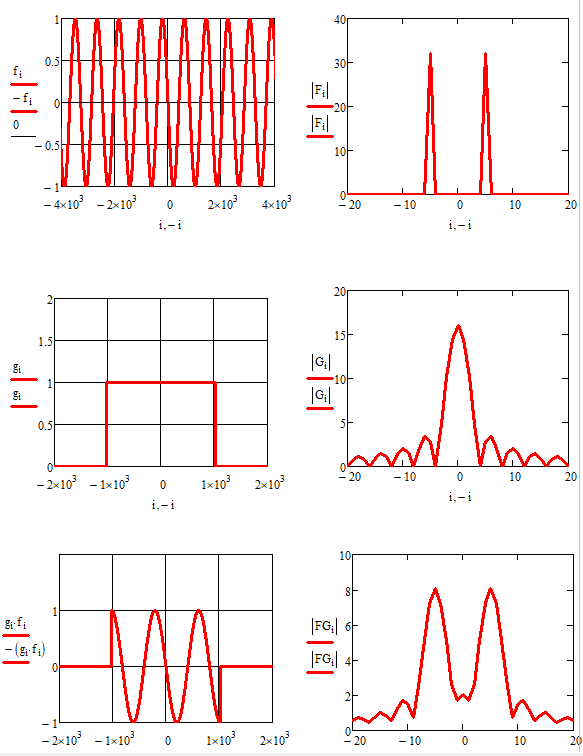
\includegraphics[scale = 0.8]{Pictures/Fourier.png}
    \caption{\centering Преобразование Фурье для функций (сверху вниз):
             1. $\sin{\left(10\pi t\right)}\quad t \in [-5\pi; 5\pi]$.
             2. Ступенька с амплитудой $1 \quad t \in [-\pi; \pi]$.
             3. Произведение функций 1 и 2.}
    \label{fig:fourier_example}
\end{figure}
Для того, чтобы понимать как работает Фурье преобразование рассмотрим графики на рис. \ref{fig:fourier_example}. Данные рисунки получены в маткаде. Качество их оставляет желать лучшего, однако автору показалось, что данный инструмент хоть и с некоторыми ограничениями, но довольно наглядно представляет предмет разговора. Читателю не стоит обращать внимание на подписи левых осей абсцисс данных графиков, поскольку они лишь симулируют используя инструмент быстрого преобразования Фурье, как работало бы настоящее преобразование Фурье для показанных функций. Далее детально разберем представленный рисунок. В левом верхнем углу изображен график функции $\sin{(10\pi t)}$, то есть обычная синусоида с частотой 5. При взятии ее образа Фурье по формулам (\ref{fourier_transform}) мы получим две $\delta$-линии расположенные симметрично относительно нуля на расстоянии соответствующему $i=\pm5$, то есть частоте 5. Важно понимать, что если бы частота равнялась $\nu$, то и $\delta$-линии располагались бы симметрично относительно нуля на расстоянии  $i=\pm \nu$. То есть преобразование Фурье показывает какие частоты содержатся в данной функции. Можно также провести соответствие с тем, что разложение обычной синусоиды в ряд Фурье, что очевидно, равно само себе.

Следующая функция, изображенная на рисунке - ступенька. Ее Фурье образ выглядит, как показано правее. Форма этой кривой описывается так называемой функцией Уиттикера - $\frac{\sin{x}}{x}$ (правда функция Уиттикера, вообще говоря, дискретна, однако форма частотной кривой имеет именно такое аналитическое выражение). \textbf{Положения, где частотная кривая пересекает абсциссу обратно пропорциональны длине импульса.} То есть, если бы наша ступенька была длиннее, то пик был бы уже.

Третья картинка показывает Фурье преобразование для произведения предыдущих функций и тут, на самом деле, чисто интуитивно ясно, что так оно и должно быть, однако все же стоит сказать о свертке.

Для этого рассмотрим задачу из теории вероятности: \textit{Пусть есть две случайные величины $x$ и $y$ с известными законами распределения $\rho_x(x)$ и $\rho_y(y)$. Необходимо найти распределение $\rho_z(z)$ для случайной величины $z=x+y$.}

Так как величины $x$ и $y$ независимы, то вполне очевидно, что в случае, если бы величны принимали только конкретные значения $\rho_z = \rho_x\rho_y$. То есть вероятность какого-то конкретного $z$ есть произведение вероятностей что $x$ и $y$ будут в сумме давать $z$. Но необходимо найти именно функцию $\rho_z(z)$, поэтому можем записать так:
\begin{equation*}
    \rho_x(x)\rho_y(y) = \rho_x(x)\rho_y(z -x)
\end{equation*}

Если мы проинтегрируем это выражение по $x$, то получим искомую функцию, так как фактически мы просуммируем все вероятности значений $x$ и $y$, при котором $x+y=z$:
\begin{equation*}
    \rho_z(z) = \int \rho_x(x)\rho_y(z -x)\, dx 
\end{equation*}

Интеграл такого типа называется интегралом типа свертки. Если бы мы варажали вместо $x$ величину $y$, то результат был бы тот же, что тоже, в принципе, понятно.

Одно из свойств Фурье преобразования, которое как раз используется в третьем преобразовании на рис. \ref{fig:fourier_example} как раз использует свертку:
\begin{equation}
    h(t)g(t) \xrightarrow{\mathscr{F}}H(\omega) * G(\omega)
    \label{svertka}
\end{equation}

Звездочка в выражении (\ref{svertka}) как раз обозначает свертку. То есть Фурье преобразование произведения функций есть свертка изображений этих функций.

Предыдущему примеру с распределениями вероятностей можно сопоставить простой физический пример: $x$ это может быть полезный сигнал с детектора, а $y$ шумовой сигнал. Их сумма дает величину на выходе, равную $z$.

Рассмотрим другой пример с использованием свертки. Пусть регистрируем излучение с двумя равновероятными энергетическими модами. То есть ожидаем получить спектр вида рис \ref{fig:f(x)}. Эта функция представляет собой сумму двух гауссовских пиков со средними 20 и 30 соответственно и дисперсией 10. Пусть функция отклика детектора представляет также гауссовский колокол (рис. \ref{fig:primer} a). Результирующий спектр представлен на рисунке (рис. \ref{fig:primer} б). Как видно, при малых дисперсиях функции отклика, ее форма, отличная от дельта линии слабо влияет на форму спектра, однако при значениях дисперсии соразмерных и более, чем у пиков в реальном спектре, наблюдаемый спектр будет уширяться вплоть до того, что моды будут не различимы.
\begin{figure}
    \centering
    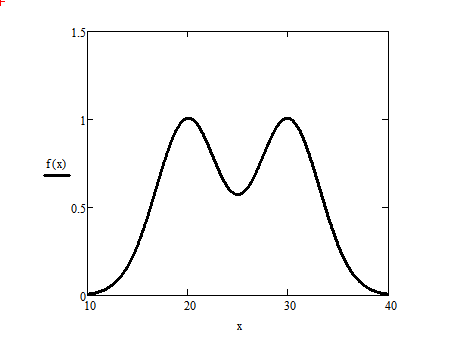
\includegraphics{Pictures/f(x).png}
    \caption{Пример измеряемого спектра.}
    \label{fig:f(x)}
\end{figure}
\begin{figure}[h]
\begin{minipage}[h]{0.49\linewidth}
\center{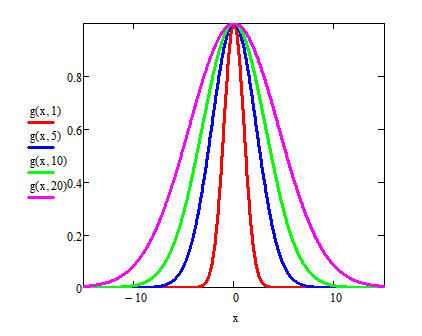
\includegraphics[scale = 0.65]{Pictures/g(x).png} \\ (а)}
\end{minipage}
\hfill
\begin{minipage}[h]{0.49\linewidth}
\center{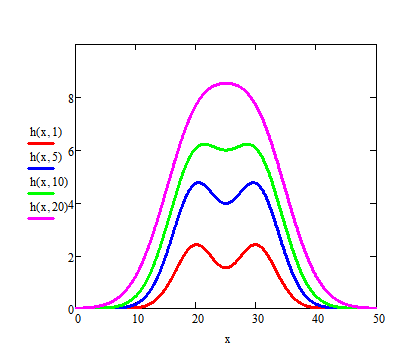
\includegraphics[scale = 0.65]{Pictures/h(x).png} \\ (б)}
\end{minipage}
\caption{Функция отклика детектора (а). Спектр на выходе детектора (б)}
\label{fig:primer}
\end{figure}

Мы уже убедились в том, что с помощью ряда Фурье можно разложить любые функции на гармонические составляющие, то есть на сумму синусов и косинусов с различными частотами. Однако в реальной жизни мы не можем раскладывать функцию в бесконечный ряд, поэтому мы вынуждены сталкиваться с некоторыми вполне закономерными ограничениями. Очевидно, что на разложение прямоугольного импульса (как на рис. \ref{fig:fourier_example} левый средний) требуется больше членов ряда, чем, например для функции отклика детектора из предыдущего примера, поскольку у первого более крутые фронты, а значит максимальная частота в его спектре разложения стремится к бесконечности, чего по факту быть не может. Поэтому все полосы пропускания различных электрических приборов и имеют гаусоподобную форму с плато вместо пика. В случае, если, все-таки, прямоугольный импульс проходит через некоторый кабель с небесконечной полосой пропускания, то в конечном итоге увидим завал фронтов нашего импульса.

Часто возникает необходимость в определении частотного состава сигнала. Это наиболее важно, когда та или иная частота несет в себе какую-либо информации через сигнал. Простой пример: наводки на детекторе. Нередко бывает так, что из-за плохого контакта с сетью, на выходе детектора сигналы выглядят не совсем так, как мы ожидаем. Можно сказать, что они выглядят "неровно". В этом случае Фурье преобразование может помочь нам определить, действительно ли дело в наводках, или нет. Об этом нам как раз скажет пик на частоте порядка $50$ Гц. 

Если в результирующем сигнале присутствуют близкие частоты, то возможность их разделения зависит от времени измерения сигнала или, как еще говоря <<временные ворота>>, то есть промежуток времени, за который мы сэмплируем сигнал. На рис. \ref{fig:rect_05} показан сигнал из трех частот 5, 20, 21 Гц соответственно, а также его Фурье спектр после измерения в течении $0.5$ секунд. 

\begin{figure}[!h]
    \centering
    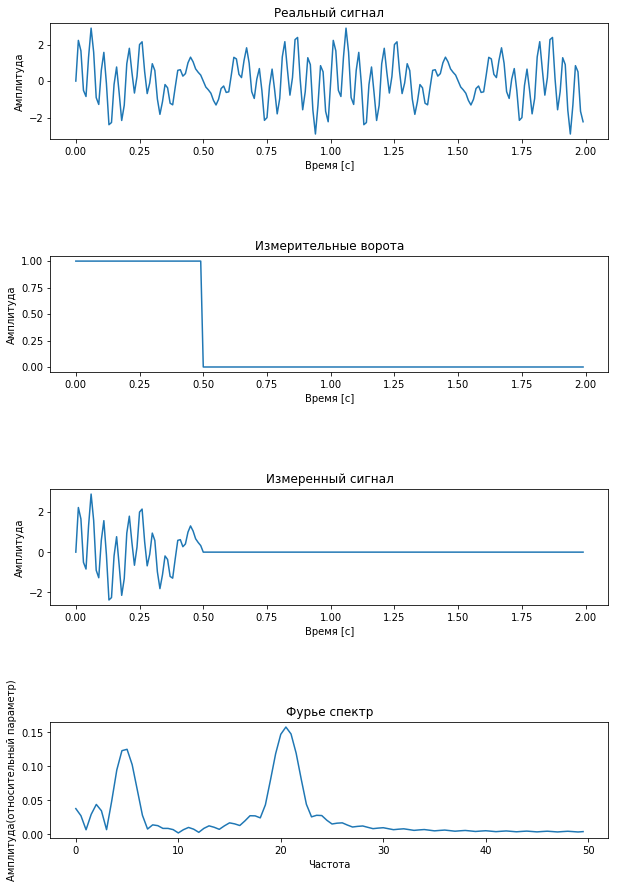
\includegraphics[scale = 0.5]{Pictures/no_separation_rectangular.png}
    \caption{Измерение сигнала и его Фурье спектр при времени измерения $0.5$ c.}
    \label{fig:rect_05}
\end{figure}

Как видим, при такой длительности измерения частоты две последние частоты не разделяются и на спектре Фурье мы видим всего один пик. Давайте посмотрим, что будет, если увеличить время измерения в два раза (рис.\ref{fig:rect_1})

\begin{figure}[!h]
    \centering
    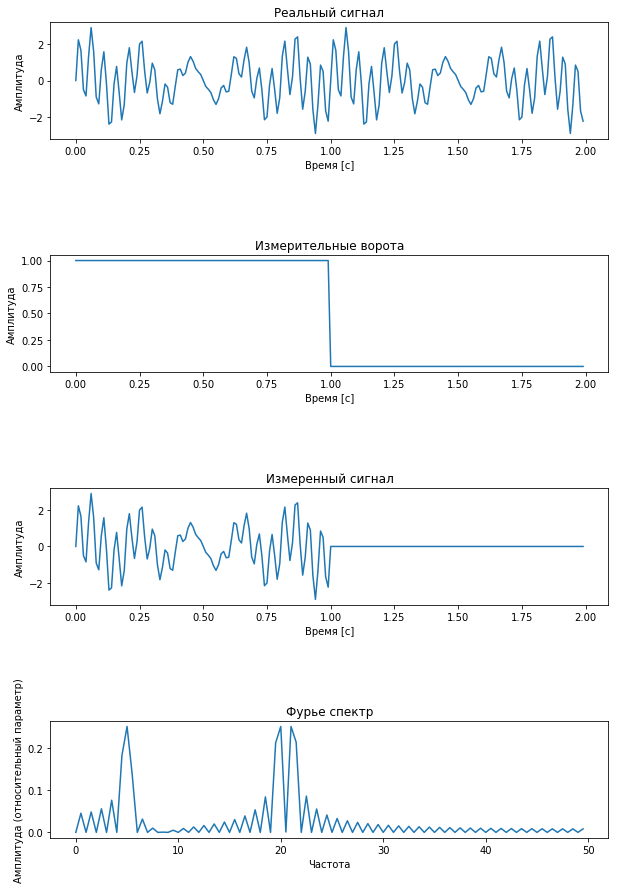
\includegraphics[scale = 0.5]{Pictures/separation_rectangular.png}
    \caption{Измерение сигнала и его Фурье спектр при времени измерения $1$ c.}
    \label{fig:rect_1}
\end{figure}

В этом случае стало хорошо видно наличие двух разделенных частот. 

Это, возможно, трудно представить, но возможны и другие формы временных окон, то есть не обязательно прямоугольные. Однако в случае с прямоугольным окном разделение частот проще, поскольку в его разложении в ряд Фурье, можно сказать, находятся все частоты, от самых малых, до бесконечно больших. Если окно, например, треугольной или гаусоподобной формы, то для разделения частот необходимо большее время измерений, поскольку фронты таких окон менее крутые, а следовательно содержат в себе более низкие частоты.

В общем и целом для различия частот необходимо выполнение следующего условия:
\begin{equation}
    T\geqslant \frac{1}{f_1 - f_2}
\end{equation}
где $T$ - ширина временного окна, а $f_1$ и $f_2$ - частоты, которые мы хотим разделить.
\section{Наложение частот}
Как мы уже говорили, в реальности нам приходится работать не с непрерывными функциями, а с дискретизированными сигналами. Понятно, что дискретизация должна происходить с какой-то частотой. Назовем эту частоту $\omega_S = \frac{2\pi}{\Delta}$, где $\Delta$ - период дискретизации. Идеальная дискретизирующая функция может быть описана рядом:
\begin{equation}
    i(t) = \sum \limits_{n = - \infty}^{+\infty} \delta\left(t - n\Delta\right)
    \label{eq:tact}
\end{equation}

Это можно интерпретировать так: через каждые $\Delta$ секунд происходит измерение нашего сигнала. Таким образом в совокупности с измеряемым сигналом на выходе мы увидим дискретную функцию, которую можно описать следующим выражением:
\begin{equation}
    s_i(t) = s(t)\cdot i(t) = s(t)\sum \limits_{n = - \infty}^{+\infty} \delta\left(t - n\Delta\right)
    \label{eq:discreted}
\end{equation}

Давайте найдем ее Фурье образ. Для этого предлагаю сначала взять Фурье образ для выражения \eqref{eq:tact}, поскольку далее мы сможем с легкостью воспользоваться свойством свертки.
Но поиск Фурье образа \eqref{eq:tact} с ходу приводит к затруднениям, поэтому можно попытаться сначала разложить ее в ряд Фурье:
\[i(t) = \frac{1}{\Delta}\sum \limits_{k = -\infty}^{+\infty} C_k e^{\frac{2\pi kt}{\Delta}}\]
коэффициенты этого ряда нетрудно ищутся:
\[C_k = \int \limits_{-\frac{\Delta}{2}}^{\frac{\Delta}{2}}e^{\frac{2\pi kt}{\Delta}}\sum \limits_{n = - \infty}^{+\infty} \delta\left(t - n\Delta\right)\,dt\]
так как в пределах интегрирования находится всего лишь одна точка с $n = 0$, то по свойству дельта функции получаем $C_k = 1$ и ряд Фурье для функции \eqref{eq:tact} выглядит следующим образом:
\begin{equation}
    i(t) = \frac{1}{\Delta}\sum \limits_{k = -\infty}^{+\infty} e^{\frac{2\pi kt}{\Delta}}
    \label{eq:Fourier_series_tact}
\end{equation}
Теперь вспомним, что  $\delta(t)\xrightarrow{\mathscr{F}}1$ и, соответственно, наоборот.
Учитывая это получаем, что:
\begin{equation}
    i(t)  \xrightarrow{\mathscr{F}} \frac{1}{\Delta}\int \limits_{-\infty}^{+\infty} \sum \limits_{n = \infty}^{+\infty} e^{-2\pi i \left(\omega - \frac{n}{\Delta}\right)}\,dt =
    \frac{1}{\Delta}\sum \limits_{n = -\infty}^{+\infty} \delta\left(\omega - \frac{n}{\Delta}\right) = I(\omega)
\label{eq:i_fourier}
\end{equation}
Учитывая, что $s_i(t) = s(t)\cdot i(t)$, то по теореме свертки Фурье образ $S_i(\omega)$:
\[S_i(\omega) = \int \limits_{-\infty}^{+\infty}S(\omega - g) I(g)\,dg\]
Подставляя \eqref{eq:i_fourier} в эту формулу, получаем:
\begin{equation}
    S_i(\omega) = \frac1{\Delta}\sum \limits_{n = -\infty}^{+\infty}S\left(\omega - \frac{n}{\Delta}\right)
\label{eq:Fourier_Si}
\end{equation}
Таким образом, зная Фурье образ для функции $s(t)$, можем утверждать, что результирующий Фурье образ будет представлять собой наложение Фурье образов $s(t)$ через каждые $\frac{1}{\Delta}$ Гц. (Надо сделать рисунок).

Отсюда видим, что наложение спектров будет зависеть от величины $\Delta$. 

Здесь мы подходим к главному принципу --- поскольку функции дискретны и кончены из-за не бесконечного периода измерений, то чем шире в одном пространстве изображение функции (временном), тем уже ее изображение в другом пространстве (частотном). Поэтому период дискретизации следует уменьшать до тех пор, пока разрешение частот (отношение $\frac1{\Delta}$) не позволит нам различать периодические структуры друг от друга.

Также необходимо отметить, что для любой реально существующей функции Фурье образ является спадающей по частоте функцией. С физической точки зрения мы можем объяснить это так: каждая частота соответствует какой-то энергии. Чем больше частота, тем больше энергия, а, как мы знаем, бесконечной энергия быть не может, следовательно и Фурье образ стремится к нулю на бесконечности для любой функции.

\section{Проблемы прямоугольного окна. Размытие спектральных составляющих.}

Как мы убедились с помощью рисунка \ref{fig:rect_1}, прямоугольное окно преобразует совокупность синусоидальных сигналов совсем не в три дельта функции, как было бы в идеале. На деле же мы видим некоторые дополнительные частоты, вклад которых, хоть и мал, но присутствует в достаточно большом (я бы даже сказал в бесконечном) диапазоне. Внимательные из вас могли догадаться (это, кстати, говорилось ранее), что данный факт связан с крутизной фронтов временного окна, то есть в результирующем спектре наблюдаются высокие частоты, отвечающие за формирование <<резких>> краев наших ворот. 

Поэтому, как правило, в качестве ворот берется функция, которая внешне очень похожа на распределение Ферми-Дирака и задается следующей формулой:
\[w(t) = \frac1{\exp\left(\frac{|t| - T}{\sigma}\right) + 1}\]
здесь параметр $T$ - отвечает за длительность ворот, $\sigma$ - за крутизну фронта. Если построить график этой функции, то можно убедиться, что единственное отличие ее от прямоугольных ворот в крутизне фронтов, поэтому варьируя ее параметры можно добиться отсутствия нежелательных высоких и низких частот. 

Чтобы еще раз показать, что крутизна фронтов действительно влияет на результирующий спектр именно таким образом, приведу рисунок \ref{fig:gaus_separation}, аналогичный \ref{fig:rect_1}, только здесь в качестве временного окна используется функция гаусса. Несмотря на то, что это не похоже на приведенную выше функцию, однако фронты все равно позволяют наблюдать тенденцию уменьшения влияния высоких частот в отличие от случая использования прямоугольного временного окна.

\begin{figure}
    \centering
    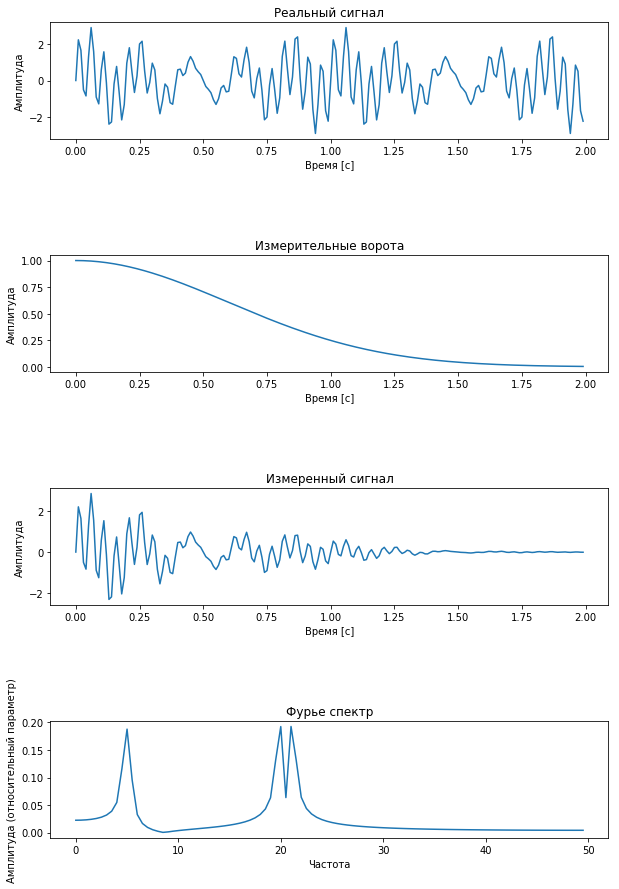
\includegraphics[scale = 0.5]{Pictures/separation_gaus.png}
    \caption{Использование временных ворот с менее крутыми фронтами.}
    \label{fig:gaus_separation}
\end{figure}

\chapter{Метод наименьших квадратов. МНК сплайн.}
\section{Важные упоминания о методе наименьших квадратов}
Здесь я не буду писать то же, что написано в любом учебнике или пособии, содержащем главу про МНК, но укажу на некоторые, может, не очевидные моменты во время разбора этой темы.

Первый, казалось бы простой, но не для всех очевидный момент, это то, что сам смысл метода кроется в его названии. Действительно, по определению вектор параметров функции $f(x, \vec \alpha)$ ищется из минимизации выражения:
\begin{equation}
    S(\alpha_1, \ldots, \alpha_k) = S(\vec \alpha) = \sum \limits_{i = 1}^{n}w_i\left[y_i - f(x, \vec \alpha)\right]^2
\end{equation}

\end{Large}
\end{document}
